% !TeX spellcheck = cs_CZ
%{\tikzset{external/prefix={tikz/FYZII/}}
% \tikzset{external/figure name/.add={ch18_}{}}
%---------------------------------------------------------------------------------------------------
% file fey2ch18.tex
%---------------------------------------------------------------------------------------------------
%====================Kapitola: Maxwellovy rovnice ==================================================
\setchaptertoc
\chapter{Maxwellovy rovnice}\label{fyz:IIchapXVIII}


  V této kapitole se vrátíme k úplnému systému čtyř Maxwellových rovnic, které pro nás byly 
  výchozím bodem v kapitole \ref{fyz:IIchapI}. Dosud jsme studovali Maxwellovy rovnice po troškách 
  a osamoceně; dozrál čas, abychom přidali poslední kousek a pak to všechno spojili. Tak dostaneme 
  úplný a pravdivý popis elektromagnetických polí, jež se mohou s časem libovolně měnit. Vše, co 
  řekneme v této kapitole a bude v rozporu s něčím, co bylo řečeno dříve, je pravda. Rozpor vzniká 
  proto, že to, co bylo řečno dříve platilo pro takové speciální případy, jakými jsou 
  např. ustálené proudy nebo nehybné náboje. Ačkoliv jsme při psaní každé rovnice velmi důsledně 
  poukazovali na omezení, tyto podmínky se snadno zapomenou a potom se naučíme nesprávné rovnice. 
  Nyní už jsme připraveni říci celou pravdu bez omezení (nebo téměř bez omezení).
  
  Úplný systém Maxwellových rovnic je zapsán v tab \ref{fyz:tab010}, a to slovy i matematickými 
  symboly. Skutečnost, že slova jsou ekvivalentní s rovnicemi by vám už měla být velmi dobře známa 
  - už by nám neměl dělat problémy překlad z jedné řeči do druhé a naopak.
  
  První rovnice - že \emph{divergence} \(\vec{E}\) je hustota náboje dělená \(\varepsilon_0\) - 
  platí obecně. \emph{Gaussův zákon} platí vždy, v případě dynamických i statických polí. 
  \emph{Tok} \(\vec{E}\) libovolnou uzavřenou plochou je úměrný náboji, který je uvnitř. Třetí 
  rovnice je odpovídající obecný zákon pro magnetická pole. Protože neexistují magnetické náboje, 
  bude tok \(\vec{B}\) libovolnou uzavřenou plochou vždy nulový. Druhá rovnice, podle níž je rotace 
  \(\vec{E}\) rovna \(-\pder{B}{T}\), je \emph{Faradayův zákon} a diskutovali jsme o ní v 
  posledních dvou kapitolách. I tato rovnice má obecnou platnost. Poslední rovnice je něčím novým. 
  Předtím jsme z ni poznali jen tu část, která platila pro stacionární proudy, a tvrdili jsme, že 
  rotace \(\vec{B}\) je rovna \(\frac{\vec{j}}{\varepsilon_0c^2}\), ale správná obecná rovnice má i 
  novou část, kterou objevil Maxwell.
  
  \begin{table}[ht!]      %\ref{fyz:tab010}
    \centering
    \begin{tabular}{l}
       \hline 
       \textbf{Maxwellovy rovnice}              \\
       \(\nabla\cdot\vec{E} = \frac{\varrho}{\varepsilon_0}\) \\
       (tok \(\vec{E}\) uzavřenou plochou) = (náboj uvnitř plochy)/\(\varepsilon_0\)  \\
       \(\nabla\times\vec{E} = -\pder{\vec{B}}{t}\)    \\
       (integral \(\vec{E}\) podél smyčky) = -\(\der{ }{t}\)(tok \(\vec{B}\) smyčkou) \\
       \(\nabla\cdot\vec{B} = 0\)                    \\
       (tok \(\vec{B}\) uzavřenou plochou)= 0        \\
       \(c^2\nabla\times\vec{B} = \frac{\vec{j}}{\varepsilon_0} + \pder{\vec{E}}{t}\) \\
       (integrál \(\vec{B}\) podél smyčky) =  (proud smyčkou)/\(\varepsilon_0\) +  \\
        + \(\der{}{t}\)(tok \(\vec{E}\) smyčkou)       \\
       \hline 
       \textbf{Zachování náboje}  \\
       \(\left[\nabla\cdot\vec{j} = -\pder{\varrho}{t}\right]\)  \\
       (tok náboje uzavřenou plochou) = -\(\der{ }{t}\)(náboj uvnitř) \\
       \hline
       \textbf{Zákon síly}  \\
       \(\vec{F} = q(\vec{E} + \vec{v}\times\vec{B})\)       \\
       \hline
       \textbf{Pohybový zákon}  \\
       \(\der{}{t}\vec{p} = \vec{F}\)  
       přičemž \(\vec{p} = \frac{m\vec{v}}{\sqrt{1-v^2/c^2}}\)   \\
       (Newtonův zákon s Einsteinovou modifikací)                 \\
       \hline
       \textbf{Gravitace}               \\
       \(\vec{F} = -\kappa\frac{m_1m_2}{r^2}\vec{e}_r\)    \\
       \hline
    \end{tabular}
    \caption{Klasická fyzika (\cite[s.~318]{Feynman02})}
    \label{fyz:tab010}
  \end{table}
    
  Zákony elektřiny a magnetizmu, známé před Maxwellovým objevem, byly předmětem našeho studia v 
  kapitolách \ref{fyz:IIchapIII} až \ref{fyz:IIchapXVII}. 
  
  Rovnice pro magnetické pole stacionárních proudů byla známa pouze v podobě
  \begin{equation}\label{fyz:eq437}
    \nabla\times\vec{B} = \dfrac{\vec{j}}{\varepsilon_0c^2}.
  \end{equation}
  
  Maxwell začal s úvahami o těch zákonech, které - podobně, jak jsme to udělalii my-vyjádřil jako 
  diferenciální rovnice. (Ačkoliv v té době ještě nebyl znám zápis pomocí \(\nabla\), je zejména 
  Maxwellovou zásluhou, že byl pochopen význam kombinací derivací, dnes známých jako rotace a 
  divergence.) Tehdy si všimnul, že s rovnicí (\ref{fyz:eq437}) není něco v pořádku. Vezmeme-li 
  divergenci této rovnice, bude levá strana nulová, neboť divergence rotace je vždy nula. Tato 
  rovnice tedy vyžaduje, aby nulová byla i divergence \(\vec{j}\). Je-li však divergence 
  \(\vec{j}\) nulová, je nulový i tok náboje libovolnou uzavřenou plochou. 
  
  Tok náboje uzavřenou plochou je roven úbytku náboje uvnitř plochy. Ten však obecně nemůže být 
  nulový, neboť víme, že náboje se mohou přemisťovat z místa na místo. Rovnice
  \begin{equation}\label{fyz:eq438}
    \nabla\cdot\vec{B} = -\pder{\varrho}{t}.
  \end{equation}
  byla téměř naší definicí \(\vec{j}\) a vyjadřuje základní zákon, že elektrický náboj se zachovává 
  - jakýkoliv tok náboje musí pocházet z nějakého zdroje. Maxwell pochopil význam tohoto problému a 
  ukázal, že ho lze odstranit přidáním členu \(\pder{\vec{E}}{t}\) na pravou stranu rovnice 
  (\ref{fyz:eq437}). Tak dostal čtvrtou rovnici v tab. \ref{fyz:tab010}:
  \begin{equation}\label{fyz:eq439}
    \text{IV}\quad c^2\nabla\times\vec{B} = \frac{\vec{j}}{\varepsilon_0} + \pder{\vec{E}}{t}.
  \end{equation}
  
  V Maxwellově době nebylo běžné uvažovat v pojmech abstraktních polí. Maxwell používal v diskuzích 
  o svých myšlenkách model, v němž bylo vakuum chápáno jako pružná pevná látka. I význam své nové 
  rovnice se snažil vysvětlit na mechanickém modelu. Jeho teorie nebyla přijata s velkou ochotou, 
  především pro použitý model, ale i proto, že nebyla zpočátku experimentálně ověřena. Dnes už 
  chápeme, že cenné jsou samotné rovnice, a ne model, který byl použit k jejich získání. Nám už 
  nezbývá nic jiného, než se ptát, zda tyto rovnice jsou správné nebo nesprávné. Odpovědí na tuto 
  otázku je nesčetné množství experimentů, které potvrdily správnost Maxwellových rovnic. 
  Odstraníme-li lešení použité na stavbě, zjistíme, že Maxwellova nádherná budova stojí na dobrých 
  základech. Dal dohromady všechny zákony elektřiny a magnetizmu a vytvořil ucelenou a krásnou 
  teorii.
  
  Nyní ukážeme, že dodatečný člen je právě to, co je nutné k odstranění problému objeveného 
  Maxwellem. Vezmeme-li divergenci jeho rovnice IV v tab. \ref{fyz:tab010}, musíme dostat, že 
  divergence pravé strany je rovna nule:
  \begin{equation}\label{fyz:eq440}
    \nabla\cdot\frac{\vec{j}}{\varepsilon_0} + \nabla\cdot\pder{\vec{E}}{t} = 0.
  \end{equation}
  
  V druhém členu lze pořadí derivací podle času a souřadnic zaměnit a rovnice získá tvar
  \begin{equation}\label{fyz:eq441}
    \nabla\cdot\vec{j} + \varepsilon_0\pder{ }{t}\nabla\cdot\vec{E} = 0.
  \end{equation}
  
  První z Maxwellových rovnic však říká, že divergence \(\vec{E}\) je rovna 
  \(\varrho\varepsilon_0\). Dosadíme-li tuto rovnost do (\ref{fyz:eq441}), dostaneme se zpět k 
  rovnici (\ref{fyz:eq438}), o níž už víme, že je správná. Naopak přijmeme-li Maxwellovy rovnice, 
  což odůvodníme tím, že zatím nebyl uskutečněn experiment, který by jim odporoval, vychází nám, že 
  náboj je vždy zachován. 
  
  Fyzikální zákony nemají odpověď na otázku: „Co se stane, vznikne-li v určitém bodě najednou 
  náboj - jaké elektromagnetické děje proběhnou?“ Na tuto otázku nemůžeme dát odpověď proto, že 
  naše rovnice říkají, že něco takového se nestane. Kdyby se něco takového mělo stát, potřebovali 
  bychom nové zákony, jenže nevíme, jaké zákony by to měly být. Neměli jsme totiž možnost 
  pozorovat, jak se svět chová bez zákona zachování náboje. Podle našich rovnic, umístíme-li 
  najednou do nějakého bodu náboj, museli jsme jej odněkud přinést. V takovém případě už však 
  umíme říct, co by se mělo stát. 
  
  Když jsme do rovnice pro rotaci \(\vec{E}\) přidali nový člen, zjistili jsme, že tím je popsána 
  celá nová třída jevů. Uvidíme, že i Maxwellův malý dodatek k rovnici pro \(\nabla\times\vec{B}\) 
  má dalekosáhlé důsledky. V této kapitole se však zmíníme jen o některých z nich.
  
  
\section{Co způsobuje nový člen}\label{fyz:IIchapXVIIIsecI}
  Jako první příklad uvažujme, co se stane s kulově symetrickým radiálním rozdělením proudu. 
  Představme si malou kouli pokrytou radioaktivní látkou. Ta vyzařuje nějaké nabité částice. (Nebo 
  si můžeme představit velký blok želé s malým otvorem uprostřed, do nějž byl stříkačkou vstříknut 
  nějaký náboj a z něhož náboj pomalu vytéká.) V obou případech budeme mít proud, který je všude 
  radiální a směřuje ven. Budeme předpokládat, že má v každém směru stejnou velikost.
  
  Nechť je celkový náboj uvnitř koule s poloměrem \(r\) rovem \(Q(r)\). Je-li radiální proudová 
  hustota v téže vzdálenosti od středu rovna \(\vec{j}(r)\), požaduje rovnice (\ref{fyz:eq438}), 
  aby \(Q\) klesalo rychlostí
  \begin{equation}\label{fyz:eq442}
    \pder{Q(r)}{t} = - 4\pi r^2j(r).
  \end{equation}
  
  \begin{figure}[ht!]  %\ref{fyz:fig326}
    \centering
    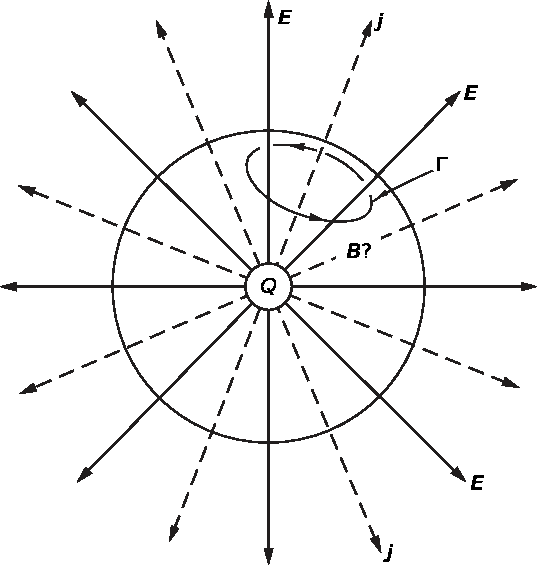
\includegraphics[width=0.7\linewidth]{fyz_fig326.pdf}
    \caption{Jaké magnetické pole má kulově symetrický proud?
             (\cite[s.~320]{Feynman02}).}
    \label{fyz:fig326}
  \end{figure}
  
  Zajímá nás, jaké je v takovémto případě magnetické pole, vytvořené proudy. Představme si, že na 
  kouli s poloměrem \(r\) je smyčka \(\Gamma\) (obr. \ref{fyz:fig326}). Touto smyčkou teče nějaký 
  proud, a proto můžeme očekávat, že v uvedeném směru bude cirkulovat magnetické pole.
  
  Dostáváme se však do problémů. Jak může mít \(\vec{B}\) nějaký určitý směr na kouli? Jiná volba 
  \(Gamma\) by nás přivedla k závěru, že má právě opačný směr. Může tam tedy vůbec nějaká cirkulace 
  \(\vec{B}\) kolem proudů být?
  
  Zachrání nás Maxwellovy rovnice. Cirkulace \(\vec{B}\) nezávisí jen na celkovém \emph{proudu} 
  tekoucím \(\Gamma\) ale i na tom, jak rychle se s časem mění \emph{elektrický tok} plochou smyčky 
  \(\Gamma\). Musí to být tak, že se tyto dva příspěvky vzájemně zruší. Podívejme se, zda tomu tak 
  opravdu je. 
  
  Předpokládáme-li, že náboj je symetricky rozložen, bude elektrické pole ve vzdálenosti \(r\) 
  rovno \(Q(r)/4\pi\varepsilon_0 r^2\). Je radiální a pro rychlost jeho změny platí
  \begin{equation}\label{fyz:eq443}
    \pder{E}{t} =  \frac{1}{4\pi\varepsilon_0 r^2}\pder{Q(r)}{t}.
  \end{equation}
  
  Porovnáme-li tento vztah se vztahem (\ref{fyz:eq442}), zjistíme, že pro libovolný poloměr platí
  \begin{equation}\label{fyz:eq444}
    \pder{E}{t} =  -\frac{\vec{j}}{\varepsilon_0}.
  \end{equation}
  
  V rovnici IV se tyto dva zdrojové členy zruší a rotace \(\vec{B}\) je vždy nulová. V našem 
  příkladu tedy magnetické pole není.
  
  Jako druhý příklad budeme uvažovat magnetické pole vodiče používaného k nabíjení deskového 
  kondenzátoru (obr. \ref{fyz:fig327}).
  
  \begin{figure}[hb!]  %\ref{fyz:fig327}
    \centering
    \subcaptionbox{\label{fyz:fig327a}}{\luafigure[0.8]{fyz_fig327a.pdf}} \\
    \subcaptionbox{\label{fyz:fig327b}}{\luafigure[0.8]{fyz_fig327b.pdf}}
    \caption{Magnetické pole v blízkosti nabíjejícího se kondenzátoru 
             (\cite[s.~321]{Feynman02}).}
    \label{fyz:fig327}
  \end{figure}
  
  Mění-li se náboj \(Q\) na deskách s časem (ale ne příliš rychle), je proud ve vodiči roven 
  \(dQ/dt\). Mohli bychom čekat, že tento proud vytvoří magnetické pole, jehož siločáry obtočí 
  vodič. Je jisté, že proud v této části vodiče, která je vzdálená od desek, vytvoří normální 
  magnetické pole - nemůže záviset na tom, kam proud teče.
  
  Předpokládejme, že máme smyčku \(\Gamma_1\), jíž je kružnice s poloměrem \(r\) znázorněná na obr. 
  \ref{fyz:fig327a}. Křivkový integrál magnetického pole by měl být roven proudu \(I\) dělenému 
  \(\varepsilon_0c^2\). Tak máme
  \begin{equation}\label{fyz:eq445}
    2\pi r B = \frac{I}{\varepsilon_0c^2}.
  \end{equation}
  
  Právě to bychom měli dostat v případě ustáleného proudu, ale souhlasí to i s Maxwellovým 
  dodatkem, protože uvažujeme-li rovinnou plochu \(S\) uvnitř kruhu, nebudou na ní elektrická pole 
  (za předpokladu, že drát je velmi dobrým vodičem). Plošný integrál \(\pder{\vec{E}}{t}\) je 
  nulový.
  
  Předpokládejme však, že nyní křivku \(\Gamma\) posouváme pomalu dolů. Budeme mít vždy stejný 
  výsledek, pokud se nedostaneme mezi desky kondenzátoru. Pak už bude proud \(I\) nulový. Zmizí tam 
  magnetické pole? To by bylo dost podivné. Všimněme si, co říkají Maxwellovy rovnice o křivce 
  \(\Gamma_2\), která je kružnicí s poloměrem \(r\) a jejíž rovina prochází mezi deskami 
  kondenzátoru (obr. \ref{fyz:fig327b}). Křivkový integrál \(\vec{B}\) podél \(\Gamma_2\) je roven 
  \(2\pi rB\). To musí být rovno časové derivaci toku \(\vec{E}\) rovinou kružnice \(S_2\). Z 
  Gaussova zákona už víme, že tento tok \(\vec{E}\) musí být roven součinu \(1/\varepsilon_0\) a 
  náboje \(Q\) na jedné z desek kondenzátoru. Máme tedy
  \begin{equation}\label{fyz:eq446}
    c^22\pi r B = \der{}{t}\left(\frac{Q}{\varepsilon_0}\right).
  \end{equation}
  
  To se nám velmi hodí. Je to tentýž výsledek, jaký představuje rovnice (\ref{fyz:eq445}). 
  Integrací přes proměnné elektrické pole dostaneme stejné magnetické pole, jako když integrujeme 
  přes proud ve vodiči. To je, samozřejmě, právě to, co říkají Maxwellovy rovnice. Snadno zjistíme, 
  že to tak musí být vždy. Stačí použít naše argumenty na dvě plochy \(S_1\) a \(S_1'\), které jsou 
  ohraničeny toutéž kružnicí \(\Gamma_1\). (obr. \ref{fyz:fig327b}). Plochou \(S_1\) teče proud 
  \(I\), ale není tam tok elektrického pole. \(S_1'\), neteče proud, ale elektrický tok se mění s 
  rychlostí \(I/\varepsilon_0\). Totéž \(\vec{B}\) dostaneme, použijeme-li rovnici IV s kteroukoliv 
  z obou ploch. 
  
  Znaší dosavadní diskuze o novém Maxwellově členu můžete získat dojem, že toho mnoho nepřidává - 
  že pouze upravuje rovnice, aby dosáhl souhlasu s tím, co už čekáme. Je pravda, že uvažujeme-li 
  samotnou rovnici IV, skutečně nic nového nedostáváme. Slova \emph{„sama o sobě“} jsou však velmi 
  důležitá. Maxwellova malá změna v rovnici IV po zkombinování s ostatními rovnicemi skutečně 
  přináší něco nového a důležitého. Dřív než o tom ale budeme hovořit, probereme více tab. 
  \ref{fyz:tab010}.
  
\section{Vše z klasické fyziky}\label{fyz:IIchapXVIIIsecII}
  V tab. \ref{fyz:tab010} máme vše, co bylo známo ze základní klasické fyziky, tj. fyziky, kterou 
  lidstvo znalo roku 1905. Máme to tu vše v jedné tabulce. Pomocí těchto rovnic můžeme pochopit 
  celou oblast klasické fyziky.
  
  Nejdříve máme Maxwellovy rovnice zapsané v rozšířené i zkrácené matematické formě. Pak je tam 
  zákon zachování náboje, který je dokonce uveden v závorkách, neboť máme-li úplný systém 
  Maxwellových rovnic, můžeme z nich zákon zachování náboje odvodit. Tabulka je tedy trochu 
  nadbytečná. Dále je tam zapsán zákon síly, neboť máme-li všechna elektrická a magnetická pole, 
  neřekne nám to nic, pokud nevíme, jak na náboje působí. Známe-li \(\vec{E}\) a \(\vec{B}\), 
  můžeme najít sílu, která působí na objekt s nábojem \(q\), pohybující se rychlostí \(v\). Znalost 
  síly nám však ještě nepoví nic, pokud nebudeme vědět, co se stane, když začne síla na něco 
  působit; potřebujeme pohybový zákon, který říká, že síla je rovna rychlosti změny hybnosti. 
  (Vzpomínáte si? Ten zákon jsme už měli v \ref{part:FYZI} díle.) V tabulce jsou zahrnuty i 
  relativistické efekty tím, že hybnost píšeme ve tvaru \(p = m_0v/\sqrt{/1 - v^2/c^2}\).
  
  Chceme-li však opravdu dosáhnout úplnosti, musíme přidat ještě jeden zákon, Newtonův gravitační 
  zákon, který jsme uvedli na konci tabulky.

  Tak máme v jedné malé tabulce všechny základní zákony klasické fyziky - máme tam ještě místo 
  na jejich slovní vyjádření a máme tam i cosi navíc. To je velká událost. Dostali jsme se velmi 
  vysoko. Obrazně řečeno, jsme na štítu K2 a jsme už téměř připraveni zdolat Mont Everest, jímž je 
  kvantová mechanika. Vyšplhali jsme na štít „Velkého Předělu“ a nyní můžeme sestoupit na druhou 
  stranu.
  
  Zejména jsme se snažili naučit, jak je třeba chápat tyto rovnice. Nyní, když už máme všechno 
  pohromadě, budeme zkoumat, co tyto rovnice znamenají, co nového říkají o tom, co ještě neznáme. 
  Museli jsme vynaložit velké úsilí, abychom se dostali až sem. Stálo nás to mnoho námahy, ale teď 
  už nás čeká příjemný sestup - nyní už budeme vidět důsledky našeho úsilí.
  
\section{Putující pole}\label{fyz:IIchapXVIIIsecIII}
  Nejdříve k novým důsledkům. Dospějeme k nim, dáme-li dohromady všechny Maxwellovy rovnice. 
  Nejdříve zjistíme, coby se mělo stát ve speciálně vybraných velmi jednoduchých podmínkách. 
  Budemc-li předpokládat, že se všechny veličiny mění pouze v jedné souřadnici, dostaneme 
  jednorozměrný problém. Situaci znázorňuje obr. \ref{fyz:fig328}. Máme nabitý list lokalizovaný v 
  rovině \(yz\). Nejdříve je list v klidu a pak náhle získá rychlost \(u\) ve směru osy \(y\) a 
  pohybuje se dál stále stejnou rychlostí. Asi nás také trápí „nekonečné“ zrychlení, ale na tom ani 
  nezáleží; stačí když si představíme, že rychlost \(u\) byla dosažena velmi rychle.

  \begin{figure}[ht!]  %\ref{fyz:fig328}
    \centering
    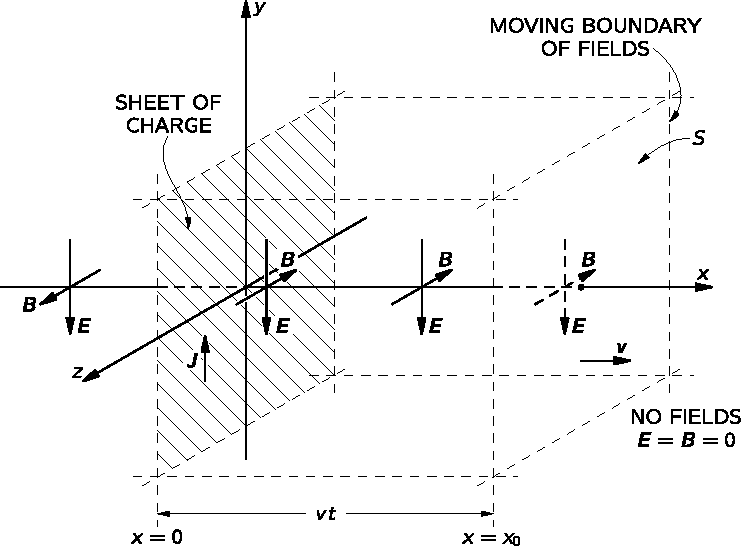
\includegraphics[width=1\linewidth]{fyz_fig328.pdf}
    \caption{Nekonečně nabitý list je náhle uveden do pohybu rovnoběžného s vlastní rovinou. Z listu
             se konstatní rychlostí šíří magnetické a elektrické pole
             (\cite[s.~323]{Feynman02}).}
    \label{fyz:fig328}
  \end{figure}

  Tak se nám najednou objevil plošný proud \(J\) (\(J\) je proud na jednotku šířky ve směru osy 
  \(z\)). Aby náš problém zůstal jednoduchý, budeme předpokládat, že na rovinu \(yz\) je 
  superponován i stacionární list plošného náboje opačného znaménka, takže nemáme elektrostatické 
  efekty. Ačkoli obrázek znázorňuje pouze to, co se děje v konečné oblasti, umíme si představit, 
  jak list prochází do nekonečna \(\pm y\) a \(\pm z\). Jinak řečeno: máme situaci, v níž nejprve 
  neteče žádný proud, a pak najednou máme celý list konstantního proudu. Co se stane?
  
  Tam, kde je list s proudem v kladném směru osy \(y\), bude, jak už víme, generováno magnetické 
  pole, které bude v záporném směru osy \(z\) pro \(x>0\) a v opačném směru pro \(x<0\). Velikost 
  \(\vec{B}\) můžeme najít, využijeme-li skutečnosti, že křivkový integrál magnetického pole bude 
  roven proudu děleném \(\varepsilon_0c^2\). Tak bychom dostali, že \(B=J/2\varepsilon_0c^2\) 
  (neboť proud I v pásu šířky \(w\) je roven \(Jw\) a křikový integrál \(\vec{B}\) je \(2Bw\)).
  
  Tak dostáváme pole v blízkosti listu, pro malé hodnoty \(x\), jenže my předpokládáme nekonečný 
  list, a proto bychom mohli čekat, že jej stejně získáme i ve velkých vzdálenostech při velkých 
  hodnotách \(x\). To by však znamenalo, že v okamžiku, kdy zapneme proud, se magnetické pole všude 
  změní z nuly na konečnou hodnotu. Ale pozor! Změní-li se náhle magnetické pole, způsobí ohromné 
  elektrické efekty. (Mění-li se \emph{jakkoliv}, máme elektrické efekty). Pohybem nabitého listu 
  jsme tedy vytvořili proměnné magnetické pole, a proto musí vzniknouti elektrická pole. 
  Vznikají-li elektrická pole, musí začít od nuly a změnit se na nějakou jinou hodnotu. Tak se 
  objeví \(\pder{\vec{E}}{t}\), které bude spolu s proudem \(J\) přispívat k tvorbě magnetického 
  pole. Protože rovnice jsou navzájem propojeny, musíme se pokusit je vyřešit najednou pro všechna 
  pole.
  
  Při pohledu na samotné Maxwellovy rovnice není snadné přímo říci, jak je třeba hledat řešení. 
  Nejdříve vám proto prozradíme řešení a na něm pak ukážeme, že opravdu vyhovuje rovnicím. Řešení 
  se zakládá na tom, že pole \(\vec{B}\), které jsme vypočítali, je vlastně generováno těsně u 
  listu s proudem (pro malé \(x\)). Musí to tak být, protože utvoříme-li uzounkou smyčku kolem 
  listu, nebude mít elektrický tok kudy projít. Pro větší hodnoty \(x\) je však pole \(\vec{B}\) 
  zpočátku nulové. Po nějakou dobu zůstává nulové a pak náhle roste. Stručně řečeno, jakmile 
  zapneme proud, dosáhne magnetické pole v jeho těsné blízkosti určité hodnoty a pak se začne šířit 
  z místa zdroje. Po určité době je všude až do určité vzdálenosti \(x\) konstantní magnetické pole 
  a ve větších vzdálenostech je pole stále nulové. V důsledku symetrie se pole šíří v kladném i 
  záporném směru osy \(x\).
 
  Pole \(\vec{E}\) se chová stejně. Předčasem \(t = 0\) (což je doba zapnutí proudu) bylo pole 
  všude nulové. Pak jsou po čase \(t=0\) pole \(\vec{E}\) i \(\vec{B}\) konstantní až od 
  vzdálenosti \(x = vt\) a nulová za touto vzdáleností. Pole se pohybují vpřed jako přílivové vlny 
  a konstantní rychlostí (ukáže se, že je to právě rychlost \(c\), ale zatím ji označujeme pouze 
  \(v\)). Graf závislostí velikostí \(\vec{E}\), resp. \(\vec{B}\) na \(x\), tak jak se jeví v 
  čase \(t\), znázorňuje obr. \ref{fyz:fig329a}.
  
  \begin{figure}[hb!] %\ref{fyz:fig329}
    \centering
    \subcaptionbox{\label{fyz:fig329a}}{\luafigure[0.8]{fyz_fig329a.pdf}}              \\
    \subcaptionbox{\label{fyz:fig329b}}{\luafigure[0.8]{fyz_fig329b.pdf}}              \\
    \subcaptionbox{\label{fyz:fig329c}}{\luafigure[0.8]{fyz_fig329c.pdf}}
    \caption{a) Velikost \(\vec{B}\) (nebo \(\vec{E}\)) jako funkce \(x\) v čase \(t\) po uvedení 
             listu do pohybu. b) Pole nabitého listu, který se začal pohybovat v čase \(t = T\) 
             směrem k záporným hodnotám \(y\). c) Součet a) a b),
             (\cite[s.~324]{Feynman02}).}
    \label{fyz:fig329}
  \end{figure}
  
  Podíváme-li se opět na obr. \ref{fyz:fig329} v čase \(t\), bude oblast mezi \(x = \pm vt\) 
  „vyplněna“ poli, ale dále už pole nezasahují. Opět zdůrazňujeme, že o nabitém listu, tedy i o 
  polích \(\vec{E}\) a \(\vec{B}\) předpokládáme, že zasahují do nekonečné vzdálenosti ve směrech 
  os \(y\) a \(z\). (Protože neumíme nakreslit nekonečnou plochu, znázornili jsme pouze to, co se 
  odehrává v konečné oblasti.)
  
  Nyní budeme kvantitativně analyzovat to, co se děje. Proto si všimneme dvou pohledů, shora podél 
  osy \(y\), který je znázorněn na obr. \ref{fyz:fig330} a bočního pohledu podél osy \(z\), který 
  je znázorněn na obr. \ref{fyz:fig331}. Nejprve začneme s bočním pohledem. Nabitý list vidíme 
  pohybovat se nahoru; magnetické pole směřuje do roviny papíru pro \(+x\) a ven z roviny papíru 
  pro \(-x\). Elektrické pole až po \(x=\pm vt\) směřuje všude dolů.

  \begin{figure}[ht!]  %\ref{fyz:fig330}
    \centering
    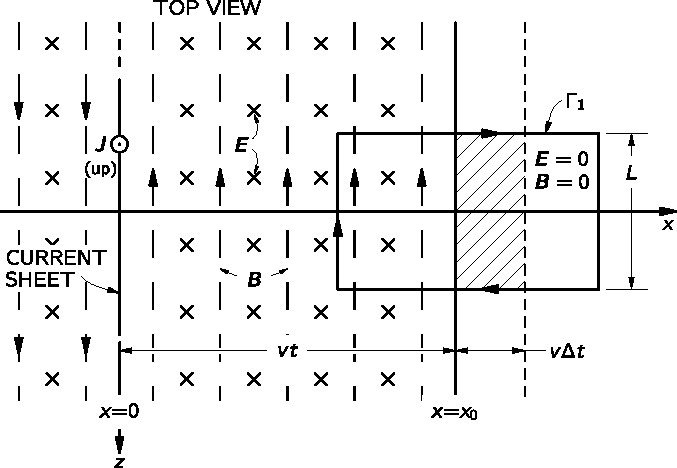
\includegraphics[width=0.9\linewidth]{fyz_fig330.pdf}
    \caption{Pohled shora k obr. \ref{fyz:fig328}
             (\cite[s.~320]{Feynman02}).}
    \label{fyz:fig330}
  \end{figure}
  
  \begin{figure}[ht!]  %\ref{fyz:fig331}
    \centering
    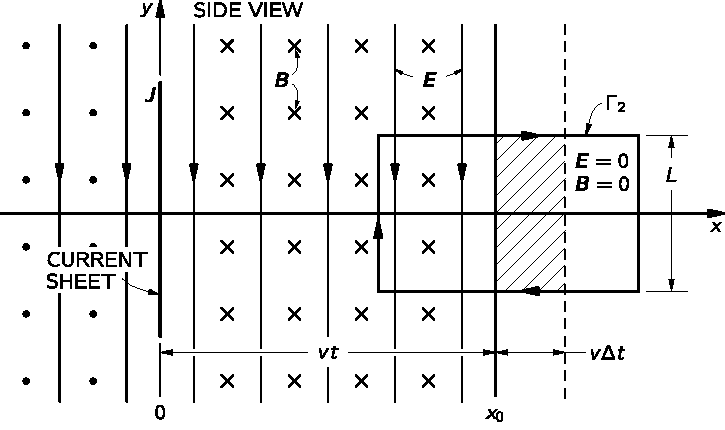
\includegraphics[width=0.9\linewidth]{fyz_fig331.pdf}
    \caption{Boční pohled k obr. \ref{fyz:fig328}
             (\cite[s.~331]{Feynman02}).}
    \label{fyz:fig331}
  \end{figure}

  Podívejme se, zda jsou tato pole konzistentní s Maxwellovými rovnicemi. Nejdříve si nakreslíme 
  jednu ze smyček, pomocí nichž jsme počítali křivkový integrál. Nechť je to pravoúhlá smyčka 
  \(\Gamma_2\): znázorněná na obr. \ref{fyz:fig331}. Všimněme si, že jedna strana pravoúhelníku je 
  v oblasti, kde existují pole a druhá je v oblasti, které pole ještě nedosáhla. Touto smyčkou 
  protéká jistý magnetický tok. Mění-li se tento tok, vytvoří se podél smyčky emn. Pohybuje-li se 
  čelo vlny, budeme mít proměnný magnetický tok, neboť plocha, v níž \(\vec{B}\) existuje, se 
  postupně zvětšuje rychlostí \(v\). Tok uvnitř je roven součinu \(\vec{B}\) a té části plochy 
  uvnitř \(\Gamma_2\)., v níž je magnetické pole. Protože velikost \(\vec{B}\) je konstantní, bude 
  rychlost změny toku rovna součinu velikosti pole a rychlosti změny plochy. Rychlost změny plochy 
  se snadno určí. Je-li šířka pravoúhelníku \(\Gamma_2\) rovna \(l\), pak plocha, v níž existuje 
  \(\vec{B}\), se mění jako \(lv\Delta t\) v čase \(\Delta t\) (obr. \ref{fyz:fig331}). Rychlost 
  změny toku je proto rovna \(Blv\). Podle Faradayova zákona to však musí být rovno křivkovému 
  integrálu \(\vec{E}\) podél \(\Gamma_2\) a ten je roven právě \(El\) Tak dostáváme rovnost
  \begin{equation}\label{fyz:eq447}
    E = vB.
  \end{equation}
  Je-li tedy poměr \(\vec{E}\) k \(\vec{B}\) roven \(v\), budou zkoumaná pole vyhovovat Faradayově 
  rovnici. 
  
  To však není jediná rovnice; máme ještě rovnici, která dává do souvislosti \(\vec{E}\) a 
  \(\vec{B}\):
  \begin{equation}\label{fyz:eq448}
    c^2\nabla\times\vec{B}  = \frac{\vec{j}}{\varepsilon_0}.+ \pder{\vec{E}}{t}
  \end{equation}
  Abychom využili této rovnice, všimneme si pohledu shora zobrazeného na obr. \ref{fyz:fig330}. Už 
  jsme viděli, že tato rovnice nám dává hodnotu \(\vec{B}\) v blízkosti nabitého listu. Také za 
  čelem vlny pro každou smyčku nebudeme mít rotaci \(\vec{B}\) ani \(\vec{j}\), ani měnící se pole 
  \(\vec{E}\), a proto tam tato rovnice bude platit. Nyní se podíváme, co se vlastně stane v křivce 
  \(\Gamma_1\), která protíná čelo vlny tak, jak je znázorněno na obr. \ref{fyz:fig330}. Nejsou zde 
  proudy a proto je možné rovnici (\ref{fyz:eq448}) vyjádřit v integrální formě
  \begin{equation}\label{fyz:eq449}
    c^2\oint_{\Gamma_1}\vec{B}\cdot\dd{\vec{s}}  = 
    \der{ }{t}\limitint_{\mathclap{\text{uvnitř }\Gamma_1}}\vec{E}\cdot\vec{n}\dd{S}.
  \end{equation}
  Křivkový integrál \(\vec{B}\) je právě součin \(B\) a \(l\). Rychlost změny toku \(E\) vzniká 
  pouze díky postupujícímu čelu vlny. Oblast uvnitř \(\Gamma_1\), kde je \(\vec{E}\) nenulové, 
  vzrůstá rychlostí \(vl\). Pravá strana rovnice (\ref{fyz:eq449}) je pak rovna \(vlE\). Rovnice 
  tedy získá tvar
  \begin{equation}\label{fyz:eq450}
    c^2B = Ev.
  \end{equation}

  Máme řešení, v němž jsou pole \(\vec{B}\) a \(\vec{E}\) za čelem vlny konstantní, obě jsou kolmá 
  ke směru postupu vlny a současně jsou kolmá navzájem. Maxwellovy rovnice určují poměr \(E\) k 
  \(B\). Z rovnic (\ref{fyz:eq447}) a (\ref{fyz:eq450}) vyplývá
  \begin{equation*}
    E = vB \quad E = \frac{c^2}{v}B.
  \end{equation*}
  
  Ale pozor! Pro poměr \(E/B\) jsme našli \emph{dvě různé} podmínky. Může pole, které jsme popsali 
  opravdu existovat? Existuje zřejmě jen jedna rychlost \(v\), pro níž jsou obě tyto rovnice 
  splněny, a pro tuto rychlost platí \(v = c\). Čelo vlny musí postupovat rychlostí \(c\). Máme 
  příklad, v němž se elektrický vliv proudu šíří určitou konečnou rychlostí \(c\). 
  
  Položme si nyní otázku, co se stane, zastavíme-li náhle pohyb nabitého listu, a to po jeho pohybu 
  v krátkém čase \(T\)? Co se stane, to se dovíme pomocí principu superpozice. Měli jsme nulový 
  proud a najednou jsme proud zapnuli. V takovém případě známe řešení. Nyní jsme rozhodnuti přidat 
  další systém polí. Vezmeme jiný nabitý list a náhle jej uvedeme do pohybu toutéž rychlostí v 
  opačném směru, ale až po čase \(T\) od začátku pohybu prvního listu. Celkový proud pocházející o 
  dobou listů je zpočátku nulový, potom se zapíná po dobu \(T\) a potom se opět vypíná, neboť se 
  oba proudy ruší. Tak máme pravoúhlý „impulz“ proudu. 
  
  Nový záporný proud vytváří stejná pole jako kladný proud, ale se všemi znaménky opačnými a s 
  časovým zpožděním \(T\). Čelo vlny opět postupuje rychlostí \(c\). V čase \(t\) dosáhlo 
  vzdálenosti \(x=\pm c(t-T)\), jak je znázorněno na obr. \ref{fyz:fig329b}. Máme tedy dva „bloky“ 
  pole postupující rychlostí \(c\), jak to znázorňuje obr. \ref{fyz:fig329a}, \ref{fyz:fig329b}. 
  Kombinovaná pole budou taková, jak je znázorňuje obr. \ref{fyz:fig329c}. Pole jsou nulová pro 
  \(x>ct\), pak jsou konstantní mezi \(x = c(t - T)\) a \(x = ct\) (s hodnotami, které jsme už 
  našli) a opět jsou nulová pro \(x<c(t-T)\). Krátce řečeno, máme malý kousek pole, blok se šířkou 
  \(cT\), který opustil proudový list a pohybuje se prostorem samostatně. Pole se „odtrhla“ a šíří 
  se volně prostorem a už nejsou spojena se zdrojem, Housenka se proměnila v motýla! 
  
  Jak může tento svazek elektrického a magnetického pole udržet sám sebe? Odpověď zní: kombinací 
  jevů pocházejících z Faradayova zákona \(\nabla\cdot\vec{E} = \pder{\vec{B}}{t}\) a nového 
  Maxwellova členu \(c^2\nabla\times\vec{B} =\pder{\vec{E}}{t}\). Pole nemají jinou možnost, než 
  se vzájemně podporovat. Předpokládejme, že magnetické pole by mělo vymizet a začalo se zmenšovat. 
  Pak by tu bylo proměnné magnetické pole, které by vytvářelo elektrické pole. Kdyby chtělo zmizet 
  toto elektrické pole, proměnné elektrické pole by opět vytvořilo magnetické pole. Neustálým 
  vzájemným působením proměnou jednoho pole v druhé - musí obě existovat stále. Nemohou 
  zmizet\footnote{ Úplně to tak není. Mohou být „absorbována“, dostanou-li se do oblasti, v níž 
  jsou náboje. Máme na mysli to, že kdesi mohou být vytvořena jiná pole, která se skládají s těmito 
  poli a „zruší“ je v důsledku destruktivní interference (viz kapitola \ref{fyz:IIchapXXXI}, 
  \ref{part:FYZI}. díl)}. Uchovávají se formou jakéhosi tance - jedno pole vytváří druhé a to druhé 
  vytváří první - a tak se šíří prostorem.

\section{Rychlost světla}\label{fyz:IIchapXVIIIsecIV}
  Máme vlnu, která opouští látkový zdroj a pohybuje se rychlostí \(c\), což je rychlost světla. 
  Vraťme se však trochu nazpět. Historie je taková, že o koeficientu \(c\) v Maxwellových rovnicích 
  nebylo známo, že je současně rychlostí šíření světla. Byla to prostě konstanta v rovnicích. My 
  jsme ji označili \(c\) hned na začátku, neboť jsme věděli, co musíme nakonec dostat. Nemyslíme 
  si, že by bylo rozumné aw vztahy s různými konstantami a pak se vrátit a dosazovat \(c\) všude 
  tam, kam patří. Z hlediska elektřiny a magnetizmu jsme však vycházeli ze dvou konstant 
  \(\varepsilon_0\) a \(c^2\), které se objevují v rovnicích elektrostatiky a magnetostatiky.
  \begin{subequations}\label{fyz:eq451}
    \begin{align}
      \nabla\cdot\vec{E}  &= \frac{\varrho}{\varepsilon_0}    \label{fyz:eq451a}\\
      \shortintertext{a} 
      \nabla\times\vec{B} &= \frac{\vec{j}}{\varepsilon_0c^2} \label{fyz:eq451b}
    \end{align}
  \end{subequations}
  Vezmeme-li libovolnou definici jednotkového náboje, můžeme experimentálně určit konstantu 
  \(\varepsilon_0\), vystupující v rovnici (\ref{fyz:eq451a}), např. měřením síly mezi dvěma 
  jednotkovými náboji v klidu s použitím Coulombova zákona. Experimentálně musíme určit i konstantu 
  \(\varepsilon_0c^2\), která se objevuje v rovnici (\ref{fyz:eq451b}). Můžeme to udělat např. 
  měřením síly působící mezi dvěma jednotkovými proudy. (Jednotkový proud znamená jednotku náboje 
  za sekundu.) Poměr těchto dvou experimentálních konstant je roven \(c^2\), což je jiná 
  elektromagnetická konstanta. 
 
  Všimněte si, že tato konstanta \(c^2\) je vždy stejná bez ohledu na to, jakou jednotku náboje 
  jsme zvolili. Zvolíme-li naší jednotkou náboje dvakrát větší náboj, např. dvakrát tolik 
  protonových nábojů, \(\varepsilon_0\) bude muset být čtyřikrát menší. Necháme-li téct takové dva 
  jednotkové proudy dvěma vodiči, proteče v každém vodiči dvakrát tolik „nábojů“ za sekundu a síla 
  mezi vodiči bude čtyřikrát větší. Konstanta \(\varepsilon_0c^2\) se musí zmenšit čtyřikrát, poměr 
  \(\varepsilon_0c^2/\varepsilon_0\), se však nemění. 
 
  Proto můžeme jen pomocí experimentů s náboji a proudy najít číslo \(c^2\), o němž se zjistilo, že 
  je druhou mocninou rychlosti šíření elektromagnetických působení. Ze statických měření (měřením 
  sil mezi dvěma jednotkovými náboji a mezi dvěma jednotkovými proudy) bychom zjistili, že 
  \(c=\SI{3.00e8}{\m/\sec}\). Když Maxwell poprvé uskutečnil tento výpočet se svými rovnicemi, mohl 
  říci, že systém elektrického a magnetického pole se bude šířit touto rychlostí. Poukázali na 
  tajemnou shodu této konstanty s rychlostí světla. „Sotva můžeme vyloučit závěr“, řekl Maxwell, 
  „že světlo je příčným vlněním téhož prostředí, které vyvolává elektrické a magnetické jevy.“ 
 
  Maxwell uskutečnil jedno z velkých sjednocení fyziky. Předním bylo světlo, jakož i elektřina a 
  magnetizmus. Elektřina a magnetizmus byly sjednoceny experimentálními pracemi Faradaye, Oersteda 
  a Ampéra. Pak náhle přestalo být světlo „něčím jiným“ a stalo se pouze elektřinou a magnetizmem v 
  nové formě - drobnými „kousky“ elektrického a magnetického pole šířícími se prostorem. 
 
  Soustředili jsme se na ty charakteristiky tohoto speciálního řešení, které se ukazují být 
  platnými pro každou elektromagnetickou vlnu: že magnetické pole je kolmé ke směru pohybu čela 
  vlny, elektrické pole je také kolmé ke směru pohybu čela vlny, a přitom jsou vektory \(\vec{E}\) 
  a \(\vec{B}\) kolmé navzájem. Dále, že velikost elektrického pole E je rovna \(c\)-násobku 
  velikosti magnetického pole \(B\).  Tyto tři skutečnosti - že obě pole jsou kolmá na směr šíření, 
  že \(\vec{B}\) je kolmé k \(\vec{E}\) a že \(E= cB\) - jsou obecně platné pro jakoukoliv 
  elektromagnetickou vlnu. Náš speciální případ je tedy dobrým příkladem; ukazuje všechny hlavní 
  vlastnosti elektromagnetických vln.
 
\section{Řešení Maxwellový rovnic. Potenciály a vlnová rovnice}\label{fyz:IIchapXVIIIsecV}
  Zkusme nyní udělat něco matematického a zapišme Maxwellovy rovnice v jednodušší formě. Zpočátku 
  se vám bude zdát, žeje komplikujeme, ale budete-li trochu trpěliví, opravdu se dočkáme jejich 
  zjednodušení. Ačkoliv jsme si už zvykli na každou Maxwellovu rovnici, je to přece jen mnoho 
  kousků a ty je třeba navzájem propojit. Právě to se chystáme udělat.
  
  Začněme se vztahem \(\nabla\cdot\vec{B}=0\), který představuje nejjednodušší z rovnic. Víme, že 
  důsledkem této rovnice je skutečnost, že \(\vec{B}\) je rotací něčeho. Zapíšeme-li tedy
  \begin{equation}\label{fyz:eq452}
    \vec{B} = \nabla\times\vec{A},
  \end{equation}
  už jsme vyřešili jednu z Maxwellových rovnic. (Mimochodem, tento vztah zůstává v platnosti i když 
  dosadíme jiný vektor \(\vec{A'}\), pro který platí \(\vec{A'} =\vec{A} +\nabla\Psi\), kde 
  \(\Psi\) je libovolné skalární pole; prostě je to proto, že rotace \(\nabla\Psi\) je nula a 
  \(\vec{B}\) se nezměnilo. O tom jsme však už hovořili.) Jako další vezměme Faradayův zákon 
  \(\nabla\times\vec{E} = - \pder{\vec{a}}{t}\), neboť ten neobsahuje žádné proudy nebo náboje. 
  Vyjádříme-li \(\vec{B}\) ve tvaru \(\nabla\times\vec{A}\) a derivujeme podle \(t\), můžeme 
  Faradayův zákon zapsat ve tvaru
  \begin{equation*}
    \nabla\times\vec{E} = - \pder{}{t}\nabla\times\vec{A}.
  \end{equation*}
  Protože sled derivací můžeme zaměnit, dá se tato rovnice vyjádřit ve tvaru
  \begin{equation}\label{fyz:eq453}
    \nabla\left(\vec{E} + \pder{\vec{A}}{t}\right).
  \end{equation}
  Vidíme, že \(\vec{E} + \pder{\vec{A}}{t}\) je vektor jehož rotace je rovna nule. Proto je tento 
  vektor gradientem něčeho. Když jsme se zabývali elektrostatikou, měli jsme \(\nabla\times\vec{E} 
  = 0\) a zjistili jsme, že samotné \(\vec{E}\) je gradientem čehosi. Považovali jsme to za 
  gradient \(-\varphi\) (minus je jen věcí dohody). Udělejme nyní totéž s \(\vec{E} + 
  \pder{\vec{A}}{t}\), a dostaneme
  \begin{equation}\label{fyz:eq454}
    \vec{E} + \pder{\vec{A}}{t} = \nabla\varphi.
  \end{equation}  
  Používáme tentýž symbol \(\varphi\), neboť v elektrostatickém případě, kdy se s časem nic nemění 
  a člen \(\pder{\vec{A}}{t}\) vymizí, bude \(\vec{E}\) naším starým \(-\nabla\varphi\). Faradayovu 
  rovnici tedy můžeme vyjádřit ve tvaru
  \begin{equation}\label{fyz:eq455}
    \vec{E} = - \nabla\varphi - \pder{\vec{A}}{t}.
  \end{equation} 
  Už jsme vyřešili dvě Maxwellovy rovnice a zjistili jsme, že k popisu elektromagnetických polí 
  \(\vec{E}\) a \(\vec{B}\) potřebujeme čtyři potenciálové funkce: skalární potenciál \(\varphi\) a 
  vektorový potenciál \(\vec{A}\), který představuje další tři funkce.
  
  Protože \(\vec{A}\) určuje část vektoru \(\vec{E}\) a také vektoru \(\vec{B}\), zajímá nás, co se 
  stane, změníme-li \(\vec{A}\) na \(\vec{A'} =\vec{A} +\nabla\Psi\)? Obecně se \(\vec{E}\) změní, 
  pokud neuděláme nějaké speciální opatření. Přece však můžeme uskutečnit 
  takovou změnu aniž bychom ovlivnili pole \(\vec{E}\) a \(\vec{B}\) (tj. aniž bychom změnili 
  fyzikální podstatu), měníme-li \(\vec{A}\) i \(\varphi\) \emph{současně} podle pravidel
  \begin{equation}\label{fyz:eq456}
    \vec{A'} =\vec{A} +\nabla\Psi, \quad \varphi = \varphi - \pder{\Psi}{t}.
  \end{equation} 
  Pak se ani \(\vec{E}\), ani \(\vec{B}\) získané z rovnice (\ref{fyz:eq455}) nezmění. Předtím jsme 
  volili \(\nabla\cdot\vec{A} = 0\), abychom zjednodušili rovnice statického případu. Nyní už to 
  tak dělat nebudeme a volbu provedeme jinak. Hned prozradíme, jaká to bude volba, neboť později se 
  stane zřejmým, proč jsme museli udělat právě takový výběr. 
  
  Vraťme se nyní k posledním dvěma Maxwellovým rovnicím, které nám poskytnou vztahy mezi potenciály 
  a zdroji \(\varrho\) a \(\vec{j}\). Budeme-li moci určit \(\vec{A}\) a \(\varphi\) z proudů a 
  nábojů, dostaneme \(\vec{E}\) a \(\vec{B}\) z rovnic (\ref{fyz:eq452}) a (\ref{fyz:eq455}), takže 
  budeme mít jinou formu Maxwellových rovnic. 
  
  Začneme tím, že vztah (\ref{fyz:eq455}) dosadíme do \(\nabla\vec{E} = \varrho/\varepsilon_0\), a 
  tak dostaneme
  \begin{equation}\label{fyz:eq457}
    \nabla\left(-\nabla\varphi + \pder{\vec{A}}{t}\right) = \frac{\varrho}{\varepsilon_0}.
  \end{equation}  
  Tento vztah můžeme psáti ve tvaru
  \begin{equation}\label{fyz:eq458}
    -\nabla^2\varphi + \pder{ }{t}\nabla\cdot\vec{A} = \frac{\varrho}{\varepsilon_0},
  \end{equation}
  který představuje jednu z rovnic dávajících \(\varrho\) a \(\vec{A}\) do souvislosti se zdroji. 
  
  Naše závěrečná rovnice bude nejsložitější. Začneme přepsáním čtvrté Maxwellovy rovnice do
  \begin{equation}\label{fyz:eq459}
    c^2\nabla\vec{B} - \pder{\vec{E}}{t} = \frac{\vec{j}}{\varepsilon_0},
  \end{equation}
  a vyjádřením \(\vec{B}\) a \(\vec{E}\) pomocí potenciálů. Použijeme k tomu rovnice 
  (\ref{fyz:eq452}) a (\ref{fyz:eq455}) a dostaneme
  \begin{equation}\label{fyz:eq460}
    c^2\nabla(\nabla\times\vec{A}) - \pder{ }{t}\left(- \nabla\varphi - \pder{\vec{A}}{t}\right) 
      = \frac{\vec{j}}{\varepsilon_0},
  \end{equation}
  První člen můžeme upravit použitím algebraické identity: \(\nabla\times(\nabla\times\vec{A}) = 
  \nabla(\nabla\cdot\vec{A})- \nabla^2\vec{A}\). Tak dostane
  \begin{equation}\label{fyz:eq461}
    c^2\nabla^2\vec{A} + c^2\nabla(\nabla\cdot\vec{A}) + \pder{ }{t}\nabla\varphi + 
    \pder{A^2}{t^2}  = \frac{\vec{j}}{\varepsilon_0},
  \end{equation}
  což není příliš jednoduché.
  
  Nyní však naštěstí můžeme využít možnosti libovolné volby divergence \(\vec{A}\). To, co se 
  chystáme udělat, je vlastně taková volba, při které separujeme rovnice pro \(\vec{A}\) a pro 
  \(\varphi\) a dáme jim stejnou formu. Můžeme to udělat tak, že vezmeme\footnote{Volba 
  \(\nabla\cdot\vec{A}\) se nazývá kalibrace. Změna \(\vec{A}\) přidáním \(\nabla\Psi\) se nazývá 
  kalibrační transformace. Rovnice (\ref{fyz:eq461}) se nazývá Lorentzova kalibrační podmínka.}
  \begin{equation}\label{fyz:eq462}
    \nabla\cdot\vec{A} = -\frac{1}{c^2}\pder{\varphi}{t}.
  \end{equation}
  Když to uděláme, dva prostřední členy \(\vec{A}\) a \(\varphi\) v rovnici (\ref{fyz:eq461}) se 
  zruší a rovnice se velmi zjednoduší: 
  \begin{equation}\label{fyz:eq463}
    \nabla^2\cdot\vec{A} - \frac{1}{c^2}\ppder{\vec{A}}{t} = - \frac{\vec{j}}{\varepsilon_0c^2}.
  \end{equation} 
  Naše rovnice pro \(\varphi\) (tj. rovnice (\ref{fyz:eq458}) získá stejný tvar
  \begin{equation}\label{fyz:eq464}
    \nabla^2\varphi - \frac{1}{c^2}\ppder{\vec{\varphi}}{t} = - \frac{\varrho}{\varepsilon_0}.
  \end{equation} 

  Jaká krásná soustava rovnic! Jejich krása spočívá především v tom, že jsou pěkně odděleny - s 
  hustotou náboje se spojuje \(\varphi\), s proudem zase \(\vec{A}\). Ačkoliv levá strana vypadá 
  trochu legračně (obsahuje operátor \(\nabla\) a \(\pder{}{t^2}\)), situace se změní, když ji 
  rozepíšeme:
  \begin{equation}\label{fyz:eq465}
    \ppder{\varphi}{x} + \ppder{\varphi}{y} + \ppder{\varphi}{z} - \frac{1}{c^2}\ppder{\varphi}{t}
      = - \frac{\varrho}{\varepsilon_0}
  \end{equation} 
  Teď už má rovnice pěknou symetrii v \(x\), \(y\), \(z\), \(t\), faktor \(-1/c^2\) je 
  nevyhnutelný, neboť čas a prostor se liší - mají různé jednotky. Maxwellovy rovnice nás přivedly 
  k novému druhu rovnic pro potenciály \(\varphi\) a \(\vec{A}\), ale ke stejnému matematickému 
  tvaru pro všechny naše čtyři funkce \(\varphi\), \(A_x\), \(A_y\), \(A_z\). Když se tyto rovnice 
  naučíme řešit, dostaneme \(\vec{B}\) a \(\vec{E}\) a \(\nabla\times\vec{A}\) a \(-\nabla\varphi - 
  \pder{\vec{A}}{t}\). Máme jinou formu elektromagnetických zákonů - jsou úplně rovnocenné s 
  Maxwellovými rovnicemi, avšak v mnoha případech se s nimi pracuje snáze než s Maxwellovými 
  rovnicemi. My už jsme vlastně vyřešili rovnici, která byla velmi podobná rovnici 
  (\ref{fyz:eq465}). Když jsme však zkoumali zvuk v \ref{fyz:IchapXLVII} kapitole \ref{part:FYZI}. 
  dílu, měli jsme rovnici
  \begin{equation*}
    \ppder{\varphi}{x} = \frac{1}{c^2}\ppder{\varphi}{t}
  \end{equation*} 
  a viděli jsme, že popisuje šíření vln rychlostí \(c\) ve směru osy \(x\), Rovnice 
  (\ref{fyz:eq465}) je odpovídající vlnovou rovnicí v trojrozměrném případě. Můžeme proto říci, že 
  v oblastech, v nichž už nejsou náboje ani proudy, není řešením těchto rovnic \emph{nevyhnutelně} 
  nulové \(\varphi\) a \(\vec{A}\). (Ačkoli nulové \(\varphi\) a \(\vec{A}\) je jedním z možných 
  řešení.) Existují řešení, v nichž se určitý soubor \(\varphi\) a \(\vec{A}\) mění s časem, ale 
  vždy Se pohybuje dál rychlostí \(c\). Pole putují volným prostorem tak, jak to bylo v případě, 
  který jsme uvedli na začátku této kapitoly.
  
  S novým Maxwellovým členem v rovnici IV se nám podařilo napsat rovnice pole pomocí \(\vec{A}\) a 
  \(\varphi\) v podobě, která je jednoduchá a ze které je hned zřejmé, že jde o elektromagnetické 
  vlny, V některých případech je však praktičtější zůstat u původních rovnic, v nichž vystupují 
  \(\vec{E}\) a \(\vec{B}\). My však nyní tyto rovnice opustíme, neboť při našem výstupu za 
  poznáním jsme se dostali na vrcholy štítů a otevírá se nám pohled na druhou stranu, do jiných 
  údolí. Nyní uvidíme věci jinak a už se můžeme těšit na nové a úchvatné pohledy.

  
%} %tikzset
%~~~~~~~~~~~~~~~~~~~~~~~~~~~~~~~~~~~~~~~~~~~~~~~~~~~~~~~~~~~~~~~~~~~~~~~~~~~~~~~~~~~~~~~~~~~~~~~~~~
